\modeCorrection

%%%% début de la page
\renewcommand{\thesection}{\textcolor{red}{Partie \Roman{section} -}}
\renewcommand{\thesubsection}{\textcolor{red}{\Roman{section}.\arabic{subsection}}}
\renewcommand{\thesubsubsection}{\textcolor{red}{\Roman{section}.\arabic{subsection}.\alph{subsubsection}}}

\setcounter{section}{0}
\setcounter{document}{0}
\sndEnTeteTPSept

\begin{center}
\begin{mdframed}[style=titr, leftmargin=60pt, rightmargin=60pt, innertopmargin=7pt, innerbottommargin=7pt, innerrightmargin=8pt, innerleftmargin=8pt]

\begin{center}
\large{\textbf{TP 7 : Mesure de la vitesse des ondes sonores dans l'air
}}
\end{center}
\end{mdframed}
\end{center}

%\begin{tableauCompetences}
%    APP & Exploiter des explications orales pour rédiger un protocole & & & & \\
 %   \hline
  %  REA & Réaliser une série de mesures ; relever les résultats obtenus & & & & \\
   %  \hline 
    % REA & Utiliser une grandeur quotient pour déterminer le numérateur ou le dénominateur& & & & \\
     %\hline 
   % COM & Rendre compte de façon écrite & & & & \\
    %\hline
    %VAL & Analyser l’ensemble des résultats de façon critique  & & & &
%\end{tableauCompetences}


%%%% objectifs
\begin{tcolorbox}[colback=blue!5!white,colframe=blue!75!black,title=Objectifs de la séance :]
\begin{itemize}
    \item Mesurer la vitesse d’un signal sonore dans l'air ;
    \item Exploiter une série de mesures indépendantes d’une grandeur physique : moyenne et écart-type ;
    \item Écrire, avec un nombre adapté de chiffres significatifs, le résultat d’une mesure ;
    \item Comparer qualitativement un résultat à une valeur de référence ;
\end{itemize}
\end{tcolorbox}

%%%% Consignes
\begin{tcolorbox}[colback=red!5!white,colframe=red!75!black,title= Consignes :]
\begin{itemize}
    \item Faire attention au matériel lors de son utilisation ;
    \item Ne pas gêner les expériences des autres avec le bruit ambiant ;
\end{itemize}
\end{tcolorbox}

%%%% contexte

\begin{tcolorbox}[colback=orange!5!white,colframe=orange!75!black,title= Scénario:]
\begin{wrapfigure}{r}{0.4\textwidth}
\vspace{-0.6cm}
    \centering
     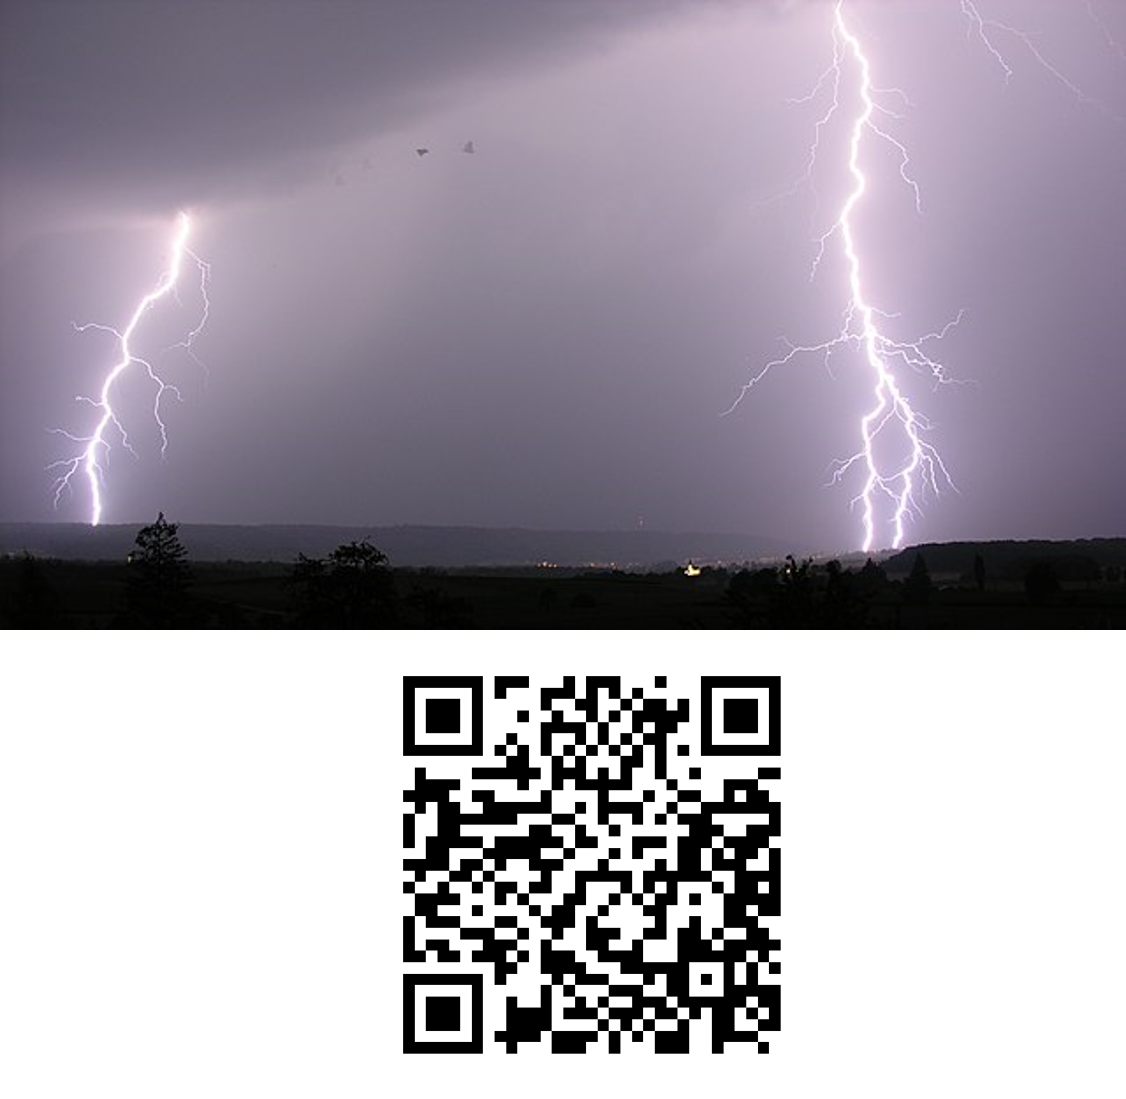
\includegraphics[width=0.4\textwidth]{Images/TP/TP7/Orage.png}
   \end{wrapfigure}
Au cours d'un orage, lorsqu'un éclair tombe à une certaine distance d'un observateur, celui-ci voit l'éclair \og immédiatement \fg~ tandis que le son du tonnerre lui parvient après quelques instants. Voici une petite vidéo qui illustre bien ce décalage : \url{https://www.youtube.com/watch?v=0XPEi0-IUtA}.\\
Le son et la lumière ne se propagent pas du tout à la même vitesse ce qui n'est pas étonnant du fait de l'origine de leur propagation : le son a besoin d'un milieu matériel (par exemple l'air, l'acier, l'eau, ...) pour se propager tandis que la lumière peut se propager dans le vide.\\

\problematique{Quelle est la vitesse de propagation du son dans l'air ?}
\end{tcolorbox}


\begin{mdframed}[style=autreexo]
\textbf{\bsc{Liste du matériel}}
\begin{itemize}
    \item Deux smartphones avec l'application Phyphox ;
    \item Une règle graduée ;
    \item Un mètre ruban de plusieurs mètres ;
    \item Un thermomètre
\end{itemize}
\end{mdframed}
 
%%%%
\newpage

\section{Mesure de la vitesse du son par Phyphox}
%%%% documents

%%%%
\begin{doc}{Protocole de mesure de la vitesse d'un signal sonore par l'application Phyphox}
\begin{wrapfigure}{r}{0.2\textwidth}
\vspace{-2cm}
    \centering
     
\includegraphics[width=0.2\textwidth]{Images/TP/TP7/qrcode_phyphox.png}
\end{wrapfigure}
Vous pouvez regarder la vidéo explicative d'un protocole de mesure de la vitesse du son dans l'air utilisant Phyphox : \url{https://www.youtube.com/watch?v=uoUm34CnHdE}.\newline
Fonctionnement du chronomètre sonore :
\begin{enumerate}
    \item Télécharger l'application Phyphox sur votre smartphone,
    \item Dans le menu principal, choisir \og Chronomètre sonore \fg ~(voir la figure de droite),
    \item Appuyer sur l'icône "Play". Relever la valeur du seuil jusqu'à ce que le chronomètre ne se déclanche plus avec le bruit ambiant de la salle,
    \item Le déclanchement du chronomètre se fait par la réception d'un son externe suffisament fort (au-dessus de la valeur du seuil) pour le smartphone et s'arrête lors de la réception d'un deuxième son suffisament fort.
\end{enumerate}

\begin{center}
    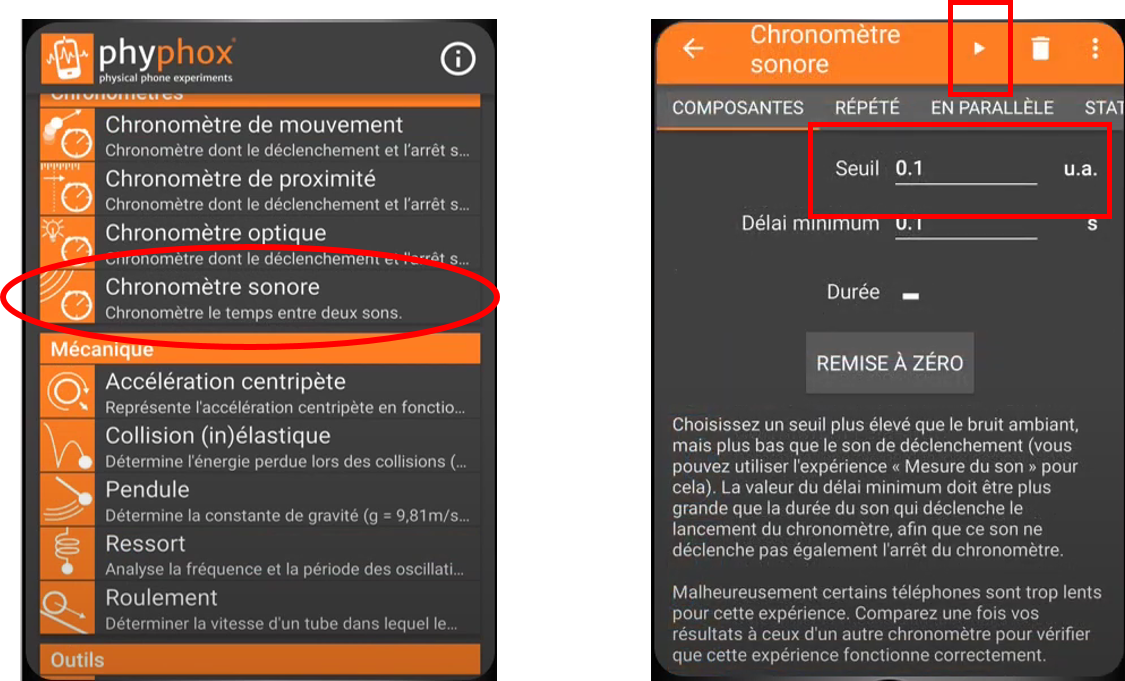
\includegraphics[scale=0.7]{Images/TP/TP7/Phyphox_1.png}
  \end{center}
\end{doc}
\newpage

\begin{doc}{\'{E}volution de la vitesse du son en fonction de la température}
Le graphe ci-dessous représente la vitesse de propagation du son dans l'air en fonction de la température de la pièce.
\begin{center}
    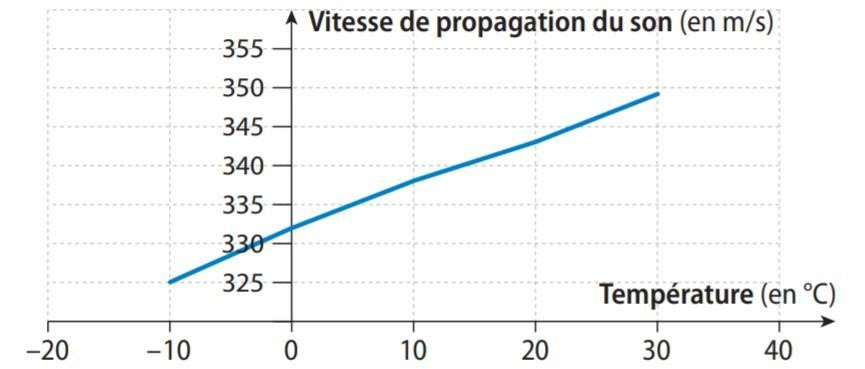
\includegraphics[scale=0.9]{Images/TP/TP7/Courbe_VitesseTemp.jpg}
  \end{center}

\end{doc}
%%%%
\begin{large}
    \textbf{\textcolor{red}{\underline{Travail à réaliser :}}}
\end{large}
\\

\question{Proposer un protocole expérimental pour mesurer la vitesse du son dans l'air.}{On a deux possibilités qui sont réalisables en pratiques :
\begin{enumerate}
    \item On place deux smartphones d'une distance $d$ suffisamment grande pour diminuer l'incertitude sur la mesure (chronomètre précis à 0,001s) et suffisamment proche pour que le son produit prêt d'un téléphone puisse être capté par l'autre téléphone ;
    \item On règle la valeur du seuil sur l'application Phyphox pour que le bruit ambiant ne déclanche pas les chronomètres sur les téléphones ;
    \item Une personne du binôme se met proche du premier smartphone et fait un premier \og clap \fg~ qui déclanche le chronomètre des deux smartphones (avec un petit décalage correspondant au temps de propagation du son entre les deux smartphones) ;
    \item L'autre personne du binôme peut ensuite faire un autre \og clap \fg~ pour arrêter les chronomètres (toujours avec le même décalage temporel) ;
    \end{enumerate}
    On aurait également pu changer la troisième et quatrième étape du protocole précédent en : 
    \begin{enumerate}
    \setcounter{enumi}{2}
        \item  Une personne du binôme se met proche du premier smartphone et fait un premier \og clap \fg~ qui déclanche le chronomètre des deux smartphones (avec un petit décalage correspondant au temps de propagation du son entre les deux smartphones) ;
        \item  L'autre personne rapproche un smartphone de l'autre sans arrêter le chronomètre puis fait un \og clap \fg~ pour arrêter simultanément les deux smartphones. 
    \end{enumerate}}{0}
%\\
\question{Faire un schéma de votre expérience, le légender et faire apparaître toutes les grandeurs physiques pertinentes : $t_{1}$ le temps mesuré par le premier smartphone, $t_{2}$ le temps mesuré par le second smartphone et $d$ la distance entre les deux smartphones.}{Merci à Lucie Keller de la 209 !\\
\begin{center}
    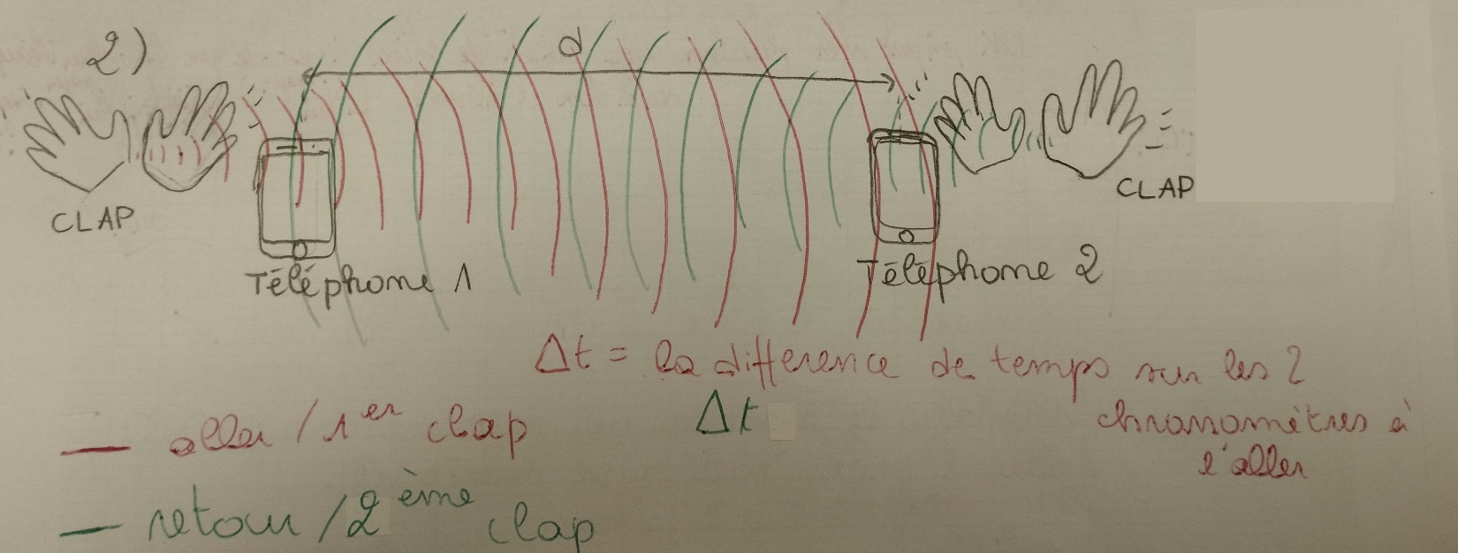
\includegraphics[scale=0.5]{Images/TP/TP7/Schema_experience.png}
\end{center}}{0} 
%\\
\question{Déterminer l'expression de la vitesse du son dans l'air, notée $c_{air}$ en fonction de $t_1$, $t_2$ et $d$.}{Le temps de parcours du son dans l'air dans l'expérience est la différence des temps mesurés par les smartphones, soit $\Delta t=t_1-t_2$. On a deux possibilités suivant l'expérience qu'on met en place :
\begin{enumerate}
    \item Si on ne change pas la distance entre les deux smartphones entre les deux signaux sonores, la distance totale que parcours le son correspond à un aller-retour entre les deux smartphones soit $2d$. La vitesse du son est donc :
        \begin{equation*}
            c_{air} = \frac{2d}{\Delta t} = \frac{2d}{t_1-t_2}
        \end{equation*}
    \item Si, après avoir fait un premier bruit, on rapproche les deux smartphones en les collant l'un à l'autre (sans arrêter le chronomètre), la distance parcourue par le son est simplement la distance $d$ donc :
    \begin{equation*}
        c_{air} = \frac{d}{\Delta t} = \frac{d}{t_1-t_2}
    \end{equation*}
\end{enumerate}}{0}
%\\
\question{Réaliser les mesures de la vitesse du son dans l'air \textbf{3 fois} et noter vos valeurs dans le tableau suivant :
\begin{center}
    \begin{tabular}{|c|C{0.25}|C{0.25}|C{0.25}|}
    \hline
         Mesures & n$^{\circ}$1 & n$^{\circ}$2 & n$^{\circ}$3 \\
         \hline
         $t_1$ (en s) & &  & \\
         \hline
         $t_2$ (en s) & &  & \\
         \hline
         $c_{air}$ (en m.s$^{-1}$) & & & \\
         \hline 
    \end{tabular}
\end{center}}{On mesure $d=2,11$~m.\begin{center}
    \begin{tabular}{|c|C{0.25}|C{0.25}|C{0.25}|}
    \hline
         Mesures & n$^{\circ}$1 & n$^{\circ}$2 & n$^{\circ}$3 \\
         \hline
         $t_1$ (en s) & 1,175 & 0,753 & 0,977 \\
         \hline
         $t_2$ (en s) & 1,164 & 0,741 & 0,967 \\
         \hline
         $c_{air}$ (en m.s$^{-1}$) & $\frac{2\times2,11}{1,175-1,164}=384$ & 325 & 422 \\
         \hline 
    \end{tabular}
\end{center}}{0}
%\\
\question{Estimer l'incertitude-type de vos mesures. \'{E}crire votre résultat expérimental sous la forme suivante :
\begin{empheq}[box=\fbox]{equation*}
    c_{air} = \text{Valeur moyenne} \pm \text{incertitude-type}
\end{empheq}}{On peut prendre par exemple l'écart entre la valeur moyenne et la valeur la plus éloignée comme incertitude. La valeur moyenne est $\frac{384+325+422}{3}=377$~m.s$^{-1}$. L'incertitude sur $c_{air}= u(c_{air})=377-325=52$~m.s$^{-1}$. On écrit donc le résultat de notre mesure :
\begin{empheq}[box=\fbox]{equation*}
    c_{air} = 377 \pm 52~\text{m.s$^{-1}$}
\end{empheq}}{0}
%\\
\question{Déterminer avec le graphique du document 2 la vitesse théorique du son dans la salle de TP. \textbf{Faire apparaître la construction graphique sur la figure.}}{\begin{center}
    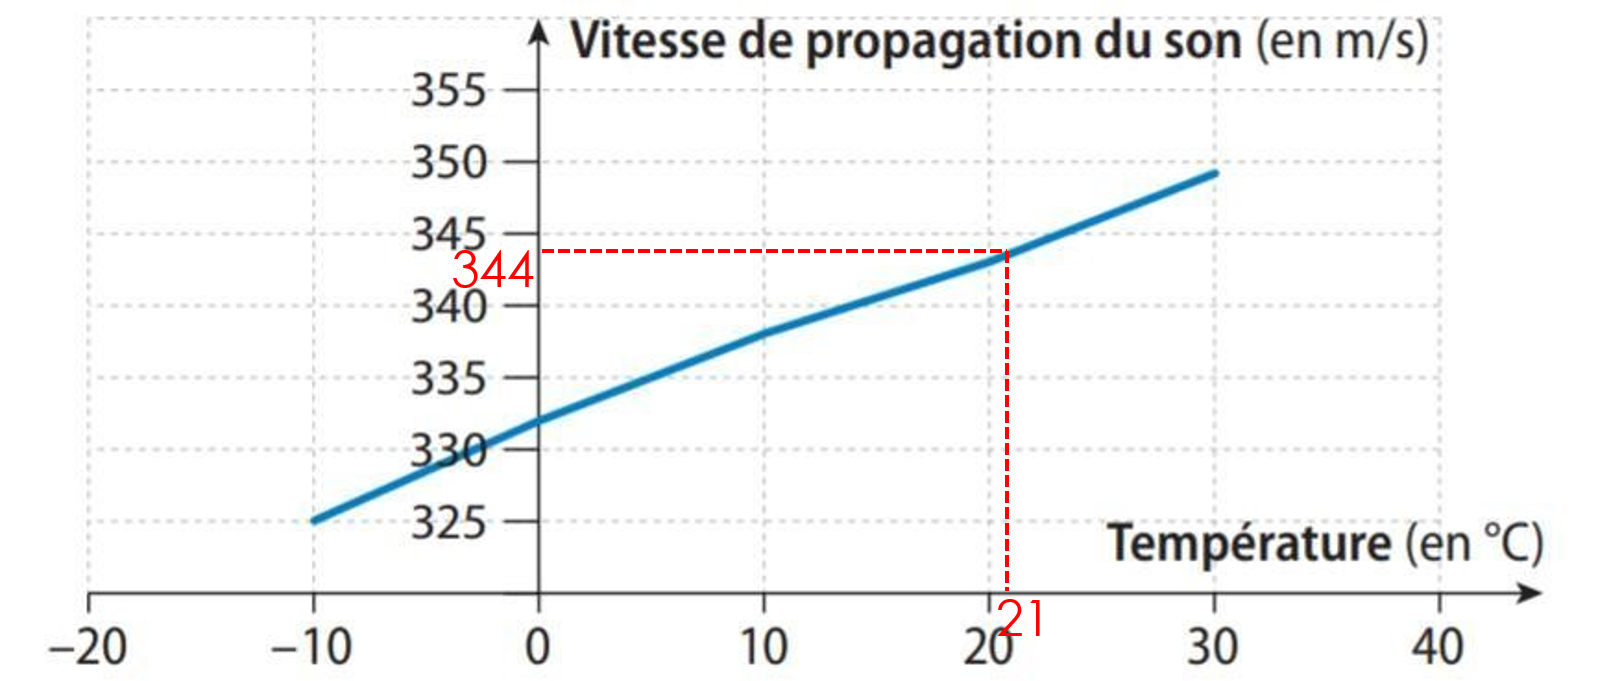
\includegraphics[scale=0.5]{Images/TP/TP7/Vitesse_son_salleTP.png}
\end{center}}{0}
%\\
\question{Votre mesure expérimentale de la vitesse de propagation du son est-elle compatible avec la valeur théorique ?}{Nos mesures nous permettent de donner un encadrement de la valeur de la vitesse du son dans l'air :
\begin{equation*}
    377-52=325\text{m.s$^{-1}$} < c_{air} < 377+52=429~\text{m.s$^{-1}$}
\end{equation*}
La valeur théorique \underline{est contenue} dans cette intervalle. On peut donc conclure que nos résultats sont compatibles avec la valeur théorique.}{0}
%\\
\question{\textit{(Bonus)} Un observateur observe un orage. L'air est lourd, le thermomètre affiche $T=25\degreCelsius$. Soudain, il voit le ciel s'éclairer et un éclair tomber. Il déclanche alors un chronomètre et mesure $\Delta t = 5,04$~s au moment où il entend le tonnerre gronder. \`{A} quelle distance de l'observateur se situe l'éclair qui vient de tomber  ?}{Comme la vitesse du son dans l'air à la température $T=25\degreCelsius$ est égale à $c(T=T=25\degreCelsius)=347$~m.s$^{-1}$, on en déduit la distance $d$ entre l'observateur et l'éclair : 
\begin{equation*}
    d = c(T=25\degreCelsius)\times \Delta t = 347\times 5 = 1,8~\text{km}
\end{equation*}}{0}

\section{\'{E}tude statistique des mesures}

\begin{doc}{\'{E}valuation d’une incertitude-type par une approche statistique}
{On l'a déjà vu au cours de l'année (TP0 et TP4) mais on peut évaluer précisément l'incertitude-type d'une grandeur physique par une approche statistique c'est-à-dire un réalisant un grand nombre de fois et de manière indépendante la même mesure de cette grandeur.\\
Si on réalise N mesures d'une grandeurs physique X (ici X=c$_{air}$), on peut calculer sa valeur moyenne , notée $\Bar{X}$, et son écart-type notée $\sigma(X)$. \\
L'incertitude-type statistique de cette grandeur X, notée $u(X)$ est alors donnée par la formule :
\begin{empheq}[box=\fbox]{equation*}
    u(X) = \frac{\sigma(X)}{\sqrt{N}}
\end{empheq}
}
\end{doc}
\begin{doc}{Représentation de la mesure statistique d'une grandeur physique et interprétation du $\pm$}
Après un grand nombre de mesures de a grandeur X en suivant un même protocole expérimental, on note le résultat final de la mesure de cette grandeur de la manière suivante :
\begin{empheq}[box=\fbox]{equation*}
    X = \Bar{X}\pm u(X) 
\end{empheq}    

où \og $\pm$ \fg~signifie plus ou moins.\\
\textbf{\textcolor{red}{Interprétation :}} Le $\pm$ signifie que si on réalise une mesure de la grandeur $X$ alors on a $68\%$ de chances que la valeur obtenue soit entre $\Bar{X}-\sigma(X)$ et $\Bar{X}+\sigma$ :
\begin{center}
    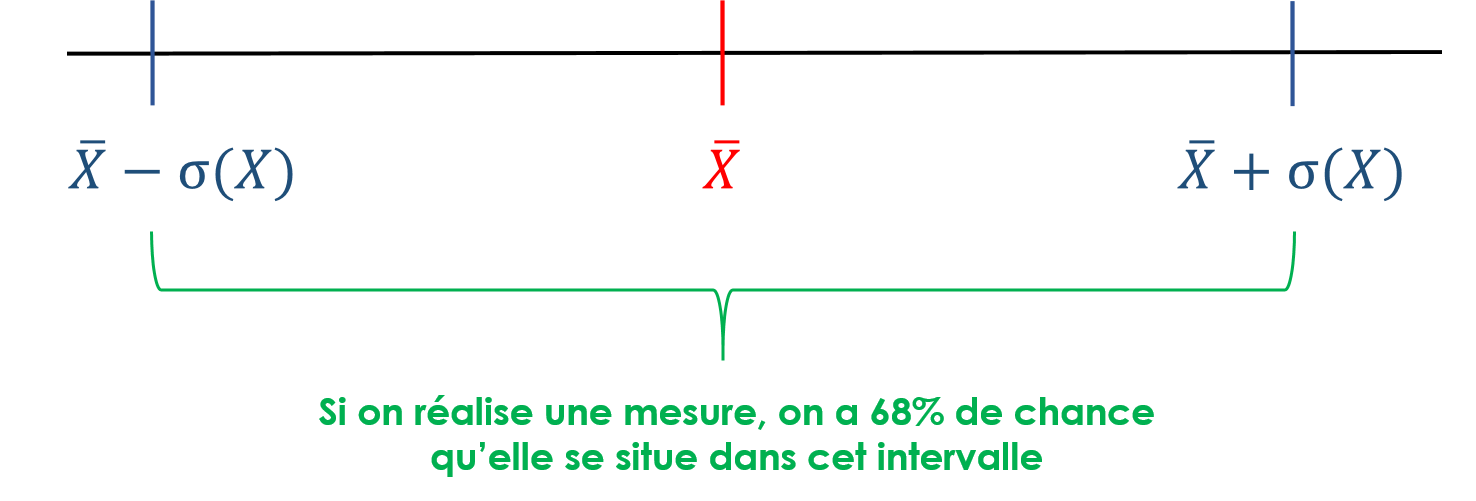
\includegraphics[scale=0.5]{Images/TP/TP7/Interpretation_sigma.png}
\end{center}
\end{doc}

\begin{large}
    \textbf{\textcolor{red}{\underline{Travail à réaliser :}}}
\end{large}
\\
\question{Récupérer le fichier \og TP7\_Resultats.xlsx \fg~dans le dossier de votre classe sur l'ENT dans l'application \og Espace Documentaire \fg. }{~}{0}
\\
\question{Rassembler tous les résultats de votre groupe dans le fichier.}{~}{0}
\\
\question{Calculer la valeur moyenne, l'écart-type ainsi que l'incertitude-type (à l'aide du document 3) à l'aide des fonctions MOYENNE, ECART-TYPE du tableur Excel.}{Voir le fichier \textit{TP7\_ResultatsGlobaux\_Classe}.}{0}
\\
\question{En utilisant le document 4, donner le résultat de la mesure statistique de $c_{air}$.}{On lit directement dans le fichier :
\begin{empheq}[box=\fbox]{equation*}
    c_{air} = 370\pm8~\text{m.s$^{-1}$}
\end{empheq}}{0}
%\\
\question{Pourquoi l'incertitude-type que vous avez estimée dans la Partie 1 est-elle plus grande que celle que vous avez obtenue par l'approche statistique ?}{D'après le document 3, plus le nombre de mesures N augmente plus l'incertitude-type diminue. Il est donc normal de trouver une incertitude estimée à la partie 1 plus grande que celle obtenue dans cette partie par une approche statistique (à part si on a fait des mesures incroyablement reproductibles mais qui sont difficilement interprétable statistiquement).}{0}
\\
\question{Le résultat du groupe est-il compatible avec la valeur théorique ? Proposer des explications possible sur la différence entre les deux.}{Explications plausibles :
\begin{itemize}
    \item Trop faible distance entre les deux téléphones, cela augmente l'erreur de mesure ;
    \item Le chronomètre sonore s'est déclanché à cause d'un bruit extérieur, la mesure peut-être faussée (en générale, cela se voit bien sur le graphe des mesures de la classe) ;
    \item La précision du chronomètre sur le téléphone est trop faible (une variation de 1ms pour une distance de 5m entre les deux téléphones donne une variation de $23$~m.s$^{-1}$ sur la vitesse de propagation du son ;
    \item Une mauvaise mesure de la distance entre les téléphones ;
\end{itemize}}{0}